% ============================================================================
%  EHD推進 空飛ぶ車 実現ロードマップ
% ============================================================================
\documentclass[12pt,a4paper]{ltjsarticle}

\usepackage{luatexja-fontspec}
\setmainjfont{HaranoAjiMincho-Regular}[BoldFont=HaranoAjiMincho-Bold]
\setsansjfont{HaranoAjiGothic-Medium}[BoldFont=HaranoAjiGothic-Bold]

\usepackage{amsmath,amssymb}
\usepackage{graphicx}
\usepackage{hyperref}
\usepackage[margin=2cm]{geometry}
\usepackage{booktabs}
\usepackage{colortbl}
\usepackage{enumitem}
\usepackage{xcolor}
\usepackage{tcolorbox}
\usepackage{fancyhdr}
\usepackage{tikz}
\usetikzlibrary{arrows.meta,shapes.geometric,positioning,calc,decorations.pathmorphing}

\tcbuselibrary{skins,breakable}

% Color definitions
\definecolor{phase0}{RGB}{149,165,166}
\definecolor{phase1}{RGB}{52,152,219}
\definecolor{phase2}{RGB}{46,204,113}
\definecolor{phase3}{RGB}{230,126,34}
\definecolor{phase4}{RGB}{231,76,60}
\definecolor{phase5}{RGB}{142,68,173}
\definecolor{phase6}{RGB}{44,62,80}
\definecolor{info}{RGB}{0,123,255}
\definecolor{success}{RGB}{40,167,69}
\definecolor{warning}{RGB}{255,193,7}
\definecolor{danger}{RGB}{220,53,69}
\definecolor{keynum}{RGB}{192,57,43}

% Custom boxes
\newtcolorbox{phasebox}[2][]{
  colback=#2!6, colframe=#2!80,
  fonttitle=\bfseries\sffamily\large, title={#1}, breakable,
  before upper={\parindent=0pt}
}
\newtcolorbox{infobox}[1][]{
  colback=info!8, colframe=info!70,
  fonttitle=\bfseries\sffamily, title={#1}, breakable
}
\newtcolorbox{keybox}[1][]{
  colback=keynum!8, colframe=keynum!70,
  fonttitle=\bfseries\sffamily, title={#1}, breakable
}
\newtcolorbox{warningbox}[1][]{
  colback=warning!15, colframe=warning!80!black,
  fonttitle=\bfseries\sffamily, title={#1}, breakable
}
\newtcolorbox{successbox}[1][]{
  colback=success!8, colframe=success!70,
  fonttitle=\bfseries\sffamily, title={#1}, breakable
}

\pagestyle{fancy}
\fancyhf{}
\fancyhead[L]{\sffamily\small EHD推進 空飛ぶ車 実現ロードマップ}
\fancyhead[R]{\sffamily\small v1.0}
\fancyfoot[C]{\thepage}

\begin{document}

% ============================================================================
%  TITLE PAGE
% ============================================================================
\begin{titlepage}
\centering
\vspace*{1.5cm}

{\Huge\sffamily\bfseries
EHD推進による\\[12pt]
空飛ぶ車\\[12pt]
実現ロードマップ
}

\vspace{0.8cm}

{\Large\sffamily
--- マイクロ電極アレイとFPGA GHz制御による\\
固体推進飛行体の段階的実現計画 ---
}

\vspace{1.5cm}

% Flying car conceptual diagram
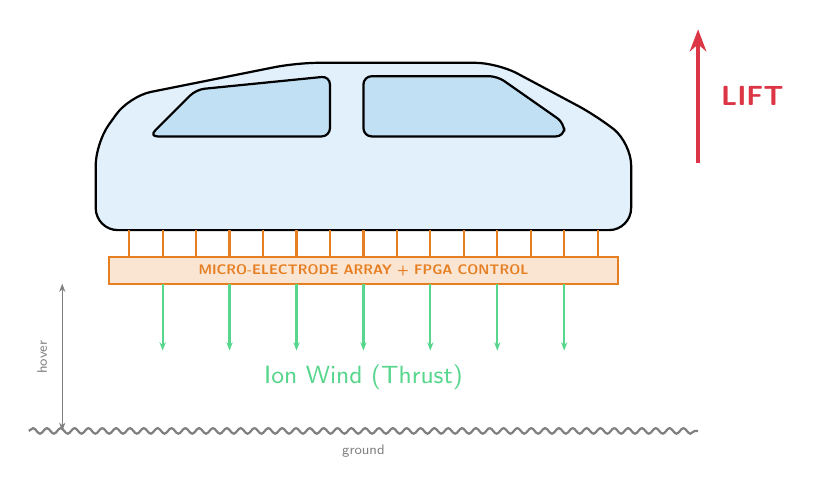
\begin{tikzpicture}[scale=0.85]
  % Car body
  \draw[thick, rounded corners=8pt, fill=phase1!15]
    (-4,-0.5) -- (-4,0.8) -- (-3.5,1.5) -- (-1,2) -- (2,2)
    -- (3.5,1.2) -- (4,0.8) -- (4,-0.5) -- cycle;

  % Windows
  \draw[thick, fill=phase1!30, rounded corners=3pt]
    (-3.2,0.9) -- (-2.5,1.6) -- (-0.5,1.8) -- (-0.5,0.9) -- cycle;
  \draw[thick, fill=phase1!30, rounded corners=3pt]
    (0,0.9) -- (0,1.8) -- (2,1.8) -- (3,1.1) -- (3,0.9) -- cycle;

  % Micro-electrode array (bottom)
  \foreach \x in {-3.5,-3.0,...,3.5} {
    \draw[phase3, thick] (\x,-0.5) -- (\x,-0.9);
  }
  \draw[phase3, thick, fill=phase3!20] (-3.8,-0.9) rectangle (3.8,-1.3);
  \node[phase3, font=\sffamily\tiny\bfseries] at (0,-1.1)
    {MICRO-ELECTRODE ARRAY + FPGA CONTROL};

  % Ion wind arrows
  \foreach \x in {-3,-2,-1,0,1,2,3} {
    \draw[-{Stealth[length=3pt]}, thick, phase2!80]
      (\x,-1.3) -- (\x,-2.3);
  }
  \node[phase2!80, font=\sffamily\small] at (0,-2.7) {Ion Wind (Thrust)};

  % Lift arrow
  \draw[-{Stealth[length=8pt]}, very thick, danger]
    (5,0.5) -- (5,2.5);
  \node[danger, font=\sffamily\bfseries, right] at (5.2,1.5) {LIFT};

  % Ground
  \draw[thick, gray, decorate, decoration={snake, amplitude=1pt, segment length=5pt}]
    (-5,-3.5) -- (5,-3.5);
  \node[gray, font=\sffamily\tiny] at (0,-3.8) {ground};

  % Height indicator
  \draw[{Stealth[length=3pt]}-{Stealth[length=3pt]}, gray]
    (-4.5,-3.5) -- (-4.5,-1.3);
  \node[gray, font=\sffamily\tiny, rotate=90] at (-4.8,-2.4) {hover};
\end{tikzpicture}

\vspace{1.5cm}

{\large\sffamily
Project: Wright Brothers \\[4pt]
\today
}

\vspace{1cm}

\begin{tcolorbox}[colback=phase1!5, colframe=phase1!50, width=12cm]
\centering\sffamily
\textbf{核心的主張：}EHD推進による空飛ぶ車は物理法則に反しない。\\
マイクロ電極アレイ（ギャップ$\sim$1\,mm）とFPGA GHz制御の組み合わせにより、\\
必要電力を既存eVTOLと同等の$\sim$200\,kWまで削減できる可能性がある。\\[4pt]
\textbf{最大の未解決問題：}効率10倍改善は達成可能か？\\
その答えを出すことが、本ロードマップの最初のゴールである。
\end{tcolorbox}

\end{titlepage}

% ============================================================================
%  TABLE OF CONTENTS
% ============================================================================
\tableofcontents
\newpage

% ============================================================================
%  SECTION 1: EXECUTIVE SUMMARY
% ============================================================================
\section{エグゼクティブサマリー}

\subsection{ビジョン}

プロペラもジェットエンジンも持たない、\textbf{完全固体推進}の空飛ぶ車を実現する。推進力は大気圧コロナ放電によるイオン風---電気流体力学（EHD）推進---のみ。可動部品ゼロ、ほぼ無音、ブレード巻き込み事故リスクなし。

\subsection{なぜ今か}

\begin{enumerate}[leftmargin=2em]
  \item \textbf{理論的枠組みの確立}: FPGA GHzフィードバック制御による動的エントロピー抑制の理論が整備された（FPGA制御論文、2026）。スケーリング則 $\mathrm{Re}_{\max} \propto \Pi_{\mathrm{ctrl}}^{2/3}$ により、制御帯域幅の増大が推力包絡線を超線形的に拡大することが証明されている。
  \item \textbf{シミュレーション技術の成熟}: JAXベースの微分可能プラズマシミュレータ（設計提案書v2.0）により、マイクロギャップ領域のスケーリング則を個人規模の計算資源で検証可能になった。
  \item \textbf{eVTOL市場の存在証明}: Joby Aviation, Lilium等がプロペラ式eVTOLの型式証明を取得しつつあり、「電動垂直離着陸」市場自体の実在が確認されている。EHDはこの市場に対して\textbf{静粛性と安全性}で差別化できる。
\end{enumerate}

\subsection{数値的根拠}

\begin{keybox}[空飛ぶ車の物理的パラメータ]
\begin{center}
\sffamily
\begin{tabular}{@{}lrl@{}}
\toprule
\textbf{パラメータ} & \textbf{値} & \textbf{備考} \\
\midrule
車両総重量 & 1,500\,kg & 車体800\,kg + バッテリー420\,kg + 乗員4名280\,kg \\
必要推力 & 15\,kN & $F = mg = 1500 \times 9.81$ \\
電極面積 & $\sim$9\,m$^2$ & 3\,m $\times$ 3\,m（車両底面・屋根面） \\
電極ギャップ & 1\,mm & マイクロ電極アレイ \\
推力密度（目標） & 1,800\,N/m$^2$ & $F \propto V^2/d^2$ スケーリングからの推算 \\
必要電力 & $\sim$187\,kW & 効率10倍改善達成時 \\
ホバリング時間 & $\sim$20分 & 75\,kWhバッテリー搭載時 \\
\bottomrule
\end{tabular}
\end{center}
\end{keybox}

% ============================================================================
%  SECTION 2: PHYSICS
% ============================================================================
\newpage
\section{物理的根拠：なぜ不可能ではないのか}

\subsection{推力密度のスケーリング}

EHD推力の体積力密度は：
\begin{equation}
  \frac{F}{V_{\mathrm{ol}}} = \rho_q E = e\, n_i\, E
  \label{eq:thrust_density}
\end{equation}

実効的な推力はドリフト領域の体積積分で得られる。電極ギャップ $d$、印加電圧 $V_0$ に対して、空間電荷制限電流の枠組み（Mott--Gurneyスケーリング）から：
\begin{equation}
  F/A \propto \frac{V_0^2}{d^2}
  \label{eq:FA_scaling}
\end{equation}

この $d^{-2}$ 依存性が、マイクロ電極アレイの核心的な利点である：

\begin{center}
\sffamily\small
\begin{tabular}{@{}cccc@{}}
\toprule
\textbf{ギャップ $d$} & \textbf{電圧 $V_0$} & \textbf{推力密度（相対値）} & \textbf{1段の厚み} \\
\midrule
30\,mm（従来） & 30\,kV & $1\times$ & 3\,cm \\
3\,mm & 3\,kV & $100\times$ & 3\,mm \\
\textbf{1\,mm} & \textbf{1\,kV} & $\mathbf{900\times}$ & \textbf{1\,mm} \\
0.3\,mm & 300\,V & $10{,}000\times$ & 0.3\,mm \\
\bottomrule
\end{tabular}
\end{center}

\subsection{効率のスケーリングとFPGA制御}

FPGA制御論文のスケーリング則：
\begin{equation}
  \mathrm{Re}_{\max} \propto \Pi_{\mathrm{ctrl}}^{2/3}, \qquad
  \Pi_{\mathrm{ctrl}} = \frac{f_{\mathrm{ctrl}}}{\gamma_{\max}/(2\pi)}
  \label{eq:scaling}
\end{equation}

ここで $f_{\mathrm{ctrl}}$ はFPGA制御帯域幅、$\gamma_{\max} \sim 10^9\,\mathrm{s}^{-1}$ は支配的不安定性成長率。

効率改善の物理的メカニズム：フィードバック制御がイオンドリフト層の\textbf{乱流遷移を遅延}させ、エネルギーが推力ではなく乱流散逸に費やされる領域を縮小する。理論的な効率改善ポテンシャル：
\begin{equation}
  \frac{\dot{S}_{\mathrm{irr}}^{\mathrm{turb}}}{\dot{S}_{\mathrm{irr}}^{\mathrm{lam}}}
  \sim \mathrm{Re}_{\mathrm{EHD}}^{1/2}
  \sim 10^2 \quad (\mathrm{Re}_{\mathrm{EHD}} \sim 10^4)
\end{equation}

すなわち、\textbf{理論上は100倍の効率改善ポテンシャル}が存在する。本ロードマップでは保守的に10倍改善を目標とする。

\subsection{電力要件の比較}

\begin{center}
\sffamily\small
\begin{tabular}{@{}lrrl@{}}
\toprule
\textbf{シナリオ} & \textbf{効率 [mN/W]} & \textbf{15\,kNに必要な電力} & \textbf{比較} \\
\midrule
制御なし（現状） & 8 & 1,875\,kW & 新幹線6両分 \\
FPGA制御（2/3乗則） & 13 & 1,150\,kW & 大型船舶 \\
FPGA + マイクロギャップ（5倍） & 40 & 375\,kW & 大型電動モーター \\
\textbf{最適制御（10倍）} & \textbf{80} & \textbf{187\,kW} & \textbf{Tesla Model 3} \\
理論上限近傍（100倍） & 800 & 19\,kW & 家庭3軒分 \\
\bottomrule
\end{tabular}
\end{center}

\begin{infobox}[既存eVTOLとの電力比較]
\sffamily
\begin{tabular}{@{}lrl@{}}
Joby Aviation S4（プロペラ式）& $\sim$200\,kW & 飛行実証済み \\
Lilium Jet（ダクテッドファン）& $\sim$1,000\,kW & 型式証明申請中 \\
\textbf{EHD空飛ぶ車（効率10倍時）} & \textbf{$\sim$187\,kW} & \textbf{シミュレーション未検証} \\
\end{tabular}

\vspace{4pt}
187\,kWは既存eVTOLと同じ電力帯。物理的に非合理ではない。
\end{infobox}


% ============================================================================
%  SECTION 3: KEY QUESTIONS
% ============================================================================
\newpage
\section{解決すべき3つの根本的問い}

本ロードマップ全体は、以下の3つの問いに段階的に答えを出す構造になっている。いずれかの問いに対する答えが「No」であれば、その時点で計画を再評価する。

\begin{keybox}[問い1（Phase 0--2で回答）]
\textbf{マイクロギャップ（$d \sim 1$\,mm）領域で、推力密度 $F/A \propto V_0^2/d^2$ のスケーリングは成立するか？}

成立しない場合の主要リスク：
\begin{itemize}[leftmargin=2em]
  \item 電極間距離が小さすぎてアーク放電（絶縁破壊）が頻発する
  \item 空間電荷効果により電流が飽和し、推力が頭打ちになる
  \item 電極表面の汚染・劣化により安定動作が維持できない
\end{itemize}
\end{keybox}

\begin{keybox}[問い2（Phase 1--3で回答）]
\textbf{FPGA GHz制御により、EHD推進効率を実際に10倍以上改善できるか？}

理論的ポテンシャルは100倍だが、実際の改善は以下に依存する：
\begin{itemize}[leftmargin=2em]
  \item マイクロギャップ領域の不安定性メカニズムがマクロスケールと同質か
  \item センサーの空間分解能がマイクロスケール不安定性を観測可能か
  \item 制御遅延（$\leq 9$\,ns）がマイクロスケール成長率に対して十分に速いか
\end{itemize}
\end{keybox}

\begin{keybox}[問い3（Phase 4--6で回答）]
\textbf{マイクロ電極アレイは実用的なサイズ（$\sim$数m$^2$）に製造可能で、長期的に安定動作するか？}

未知のリスク：
\begin{itemize}[leftmargin=2em]
  \item 大面積マイクロ電極の均一性（製造公差）
  \item ダスト・湿気による短絡リスク
  \item 電極のエロージョン（コロナ放電によるスパッタリング）
  \item オゾン・NOx生成の抑制または中和
\end{itemize}
\end{keybox}


% ============================================================================
%  SECTION 4: ROADMAP
% ============================================================================
\newpage
\section{6フェーズ・ロードマップ}

\subsection{全体像}

\begin{center}
\begin{tikzpicture}[
  pbox/.style={draw, rounded corners=6pt, minimum width=3.8cm,
    minimum height=2.2cm, font=\sffamily\small, align=center, thick},
  arr/.style={-{Stealth[length=5pt]}, thick, gray!70},
  gate/.style={diamond, draw, thick, fill=danger!20, inner sep=1pt,
    font=\sffamily\tiny\bfseries, text=danger},
  scale=0.9
]
  % Phase boxes
  \node[pbox, fill=phase0!15, draw=phase0] (p0) at (0,4)
    {\textbf{Phase 0}\\計算基盤\\構築};
  \node[pbox, fill=phase1!15, draw=phase1] (p1) at (4.5,4)
    {\textbf{Phase 1}\\スケーリング\\検証};
  \node[pbox, fill=phase2!15, draw=phase2] (p2) at (9,4)
    {\textbf{Phase 2}\\マイクロ電極\\試作};
  \node[pbox, fill=phase3!15, draw=phase3] (p3) at (0,0)
    {\textbf{Phase 3}\\ドローン\\スケール};
  \node[pbox, fill=phase4!15, draw=phase4] (p4) at (4.5,0)
    {\textbf{Phase 4}\\有人\\プロトタイプ};
  \node[pbox, fill=phase5!15, draw=phase5] (p5) at (9,0)
    {\textbf{Phase 5}\\空飛ぶ車\\実証};

  % Arrows with gates
  \draw[arr] (p0) -- (p1);
  \draw[arr] (p1) -- (p2);
  \draw[arr] (p2) -- (p3);
  \draw[arr] (p3) -- (p4);
  \draw[arr] (p4) -- (p5);

  % Go/No-Go gates
  \node[gate] at (2.25,4.9) {G1};
  \node[gate] at (6.75,4.9) {G2};
  \node[gate] at (10.2,2) {G3};
  \node[gate] at (2.25,0.9) {G4};
  \node[gate] at (6.75,0.9) {G5};

  % Labels
  \node[below, font=\sffamily\tiny, phase0] at (p0.south) {3ヶ月 / 20万円};
  \node[below, font=\sffamily\tiny, phase1] at (p1.south) {6ヶ月 / 5万円};
  \node[below, font=\sffamily\tiny, phase2] at (p2.south) {12ヶ月 / 50万円};
  \node[below, font=\sffamily\tiny, phase3] at (p3.south) {18ヶ月 / 300万円};
  \node[below, font=\sffamily\tiny, phase4] at (p4.south) {24ヶ月 / 5千万円};
  \node[below, font=\sffamily\tiny, phase5] at (p5.south) {36ヶ月+ / 数億円};

  % Gate legend
  \node[gate, minimum size=0.5cm] at (12,4.5) {};
  \node[right, font=\sffamily\tiny] at (12.4,4.5) {Go/No-Go判定};
\end{tikzpicture}
\end{center}

\begin{warningbox}[Go/No-Go ゲート]
各フェーズの境界に\textbf{Go/No-Goゲート}を設ける。ゲートの判定基準は定量的であり、達成できない場合はプロジェクトを中止するか、方針を大幅に転換する。「できないことを続ける」ことを防ぐ安全弁である。
\end{warningbox}

% ============================================================================
%  PHASE 0
% ============================================================================
\newpage
\subsection{Phase 0：計算基盤構築（3ヶ月 / 約20万円）}

\begin{phasebox}[Phase 0 --- 自宅PCでシミュレーション環境を構築し、基礎検証を行う]{phase0}
\textbf{場所：}自宅 \quad
\textbf{人員：}1名 \quad
\textbf{予算：}約200,000円（PC構築費）
\end{phasebox}

\subsubsection{目標}
\begin{enumerate}[leftmargin=2em]
  \item 自作PC（Ryzen 5 7600 + RTX 3090 24GB + 64GB RAM + Ubuntu）の構築
  \item JAX + CUDA環境の動作確認
  \item JAX-in-Cell（微分可能PIC）による1D Landau減衰の再現
  \item 論文の制御則（カルマンフィルタ + LQRゲイン）のPython行動モデル実装
  \item プラズマシミュレータとFPGA制御ロジックの結合シミュレーション
\end{enumerate}

\subsubsection{具体的タスク}

\begin{center}
\sffamily\small
\begin{tabular}{@{}cp{6cm}p{3cm}c@{}}
\toprule
\textbf{週} & \textbf{タスク} & \textbf{成果物} & \textbf{GPU使用} \\
\midrule
1--2 & 秋葉原でPC部品購入・組み立て・Ubuntu/CUDA/JAXセットアップ & 動作するPC & --- \\
3--4 & JAX-in-Cellの導入、1D Landau減衰の再現、微分可能性の確認 & 検証済みPICコード & Yes \\
5--6 & 1D EHDプラズマモデルの実装（Navier--Stokes + Maxwell結合） & EHDシミュレータ & Yes \\
7--8 & FPGA制御則のPython行動モデル実装、閉ループ結合 & 制御付きシミュレータ & Yes \\
9--10 & スケーリング則 $\mathrm{Re}_{\max} \propto \Pi_{\mathrm{ctrl}}^{2/3}$ の1D数値検証 & 検証レポート & Yes \\
11--12 & 結果分析、Phase 1計画の精緻化 & Phase 0報告書 & --- \\
\bottomrule
\end{tabular}
\end{center}

\subsubsection{PC構成（秋葉原購入リスト）}

\begin{center}
\sffamily\small
\begin{tabular}{@{}llr@{}}
\toprule
\textbf{部品} & \textbf{選定} & \textbf{価格目安} \\
\midrule
CPU & AMD Ryzen 5 7600 (6C/12T) & 28,000円 \\
マザーボード & B650 Micro-ATX & 20,000円 \\
RAM & DDR5-5600 64GB (32GB$\times$2) & 25,000円 \\
GPU & \textbf{中古 RTX 3090 24GB} & 80,000円 \\
SSD & NVMe Gen4 2TB & 18,000円 \\
電源 & 850W 80PLUS Gold & 16,000円 \\
ケース & Micro-ATX（エアフロー重視） & 7,000円 \\
OS & Ubuntu 24.04 LTS & 0円 \\
\midrule
\textbf{合計} & & \textbf{$\sim$194,000円} \\
\bottomrule
\end{tabular}
\end{center}

\subsubsection{Go/No-Go ゲート G1}

\begin{successbox}[G1通過条件]
\begin{enumerate}[leftmargin=2em]
  \item JAXベースの1D EHDシミュレータが動作し、end-to-end自動微分が可能である
  \item FPGA制御則との閉ループシミュレーションにおいて、制御帯域幅の増大が安定動作範囲を拡大することが数値的に確認できる
  \item 1Dスケーリング則 $\mathrm{Re}_{\max} \propto \Pi_{\mathrm{ctrl}}^{2/3}$ が $\pm 20\%$ 以内で再現される
\end{enumerate}
\end{successbox}

% ============================================================================
%  PHASE 1
% ============================================================================
\newpage
\subsection{Phase 1：スケーリング検証（6ヶ月 / 約5万円）}

\begin{phasebox}[Phase 1 --- マイクロギャップ領域のシミュレーション + 基礎実験]{phase1}
\textbf{場所：}自宅 \quad
\textbf{人員：}1名 \quad
\textbf{予算：}約50,000円（リフター実験 + FPGA評価ボード）
\end{phasebox}

\subsubsection{目標：問い1への回答}

シミュレーションと小規模実験の両面から、マイクロギャップ領域の推力密度スケーリングを検証する。

\subsubsection{シミュレーション（自宅PC）}

\begin{enumerate}[leftmargin=2em]
  \item \textbf{2D EHDシミュレータの構築}：Phase 0の1Dコードを2D（軸対称）に拡張。JAXのjax.checkpointを活用してVRAM管理。
  \item \textbf{ギャップスイープ}：$d = 0.3, 0.5, 1, 3, 10, 30$\,mmに対して推力密度を計算し、$F/A \propto V_0^2/d^2$ スケーリングの成立範囲を特定。
  \item \textbf{FPGA制御のマイクロスケール検証}：$d = 1$\,mm領域で不安定性成長率 $\gamma_{\max}$ を計算し、$\gamma_{\max}/(2\pi) < f_{\mathrm{ctrl}} = 1$\,GHz であることを確認。
  \item \textbf{効率改善の定量予測}：FPGA制御あり/なしの効率比を、$d$ の関数として算出。
\end{enumerate}

\subsubsection{基礎実験（自宅）}

\begin{enumerate}[leftmargin=2em]
  \item \textbf{基本リフターの製作}（実験計画書 Phase 1）：$\sim$5,000円。30mmギャップでのコロナ放電・推力発生を確認。
  \item \textbf{ギャップ変更実験}：同一電極でギャップを10, 20, 30\,mmに変えて推力を測定。$F \propto d^{-2}$ のマクロスケール検証。
  \item \textbf{Amaranth HDL評価}：FPGA制御パイプラインの行動モデルを固定小数点RTLに変換する予備実験（Arty A7-35T、$\sim$15,000円）。
\end{enumerate}

\subsubsection{Go/No-Go ゲート G2}

\begin{successbox}[G2通過条件]
\begin{enumerate}[leftmargin=2em]
  \item シミュレーションで $d = 1$\,mm において推力密度が $d = 30$\,mm の100倍以上であることが確認される（$d^{-2}$ スケーリングの成立）
  \item $d = 1$\,mm領域の不安定性成長率 $\gamma_{\max}$ が $10^{10}\,\mathrm{s}^{-1}$ 以下であり、1\,GHz FPGA制御で抑制可能である
  \item FPGA制御による効率改善が、シミュレーション上で\textbf{少なくとも3倍}確認される
  \item 基礎実験で推力がシミュレーション予測と定性的に（$\pm$ 50\%以内）一致する
\end{enumerate}
\end{successbox}

\begin{warningbox}[G2でNoの場合]
推力密度スケーリングが成立しない場合、マイクロ電極アレイ方式を断念し、以下を検討する：
\begin{itemize}[leftmargin=2em]
  \item マクロ電極の多段スタック方式（面積で稼ぐ）への方針転換
  \item 空飛ぶ車ではなく、軽量ドローン（$\sim$100\,g）を最終目標に切り替え
  \item 推進以外のEHD応用（冷却、送風、流体制御）への展開
\end{itemize}
\end{warningbox}

% ============================================================================
%  PHASE 2
% ============================================================================
\newpage
\subsection{Phase 2：マイクロ電極アレイ試作（12ヶ月 / 約50万円）}

\begin{phasebox}[Phase 2 --- マイクロ電極の試作と推力密度の実測]{phase2}
\textbf{場所：}自宅 + 大学・研究機関の共用施設（クリーンルーム等） \quad
\textbf{人員：}1--2名 \quad
\textbf{予算：}約500,000円
\end{phasebox}

\subsubsection{目標：問い1への実験的回答、問い2への着手}

\subsubsection{マイクロ電極アレイの試作}

\begin{center}
\sffamily\small
\begin{tabular}{@{}p{3cm}p{4cm}p{2cm}p{3cm}@{}}
\toprule
\textbf{タスク} & \textbf{詳細} & \textbf{費用} & \textbf{備考} \\
\midrule
PCB電極基板 & FR4基板上にCu電極パターン。ギャップ1\,mm & 50,000円 & 外注PCB製造 \\
精密スペーサー & 1\,mmアクリルシート、レーザーカット & 20,000円 & \\
高圧電源 & DC 0--5\,kV可変、安定化 & 80,000円 & \\
精密推力測定 & 電子天秤 0.001\,g + 治具 & 30,000円 & \\
FPGA制御基板 & Arty A7 + 高速ADC/DAC shield & 50,000円 & \\
センサー & 電流プローブ、電場プローブ & 80,000円 & \\
安全装備 & 絶縁手袋、放電棒、排気設備 & 50,000円 & \\
材料費 & 試作の反復分 & 40,000円 & \\
施設利用費 & 大学共用施設 & 100,000円 & \\
\midrule
\textbf{合計} & & \textbf{$\sim$500,000円} & \\
\bottomrule
\end{tabular}
\end{center}

\subsubsection{測定項目}
\begin{enumerate}[leftmargin=2em]
  \item 推力密度 $F/A$ vs ギャップ $d$（0.5, 1, 2, 3\,mm）
  \item 推力密度 $F/A$ vs 印加電圧 $V_0$（100\,V--5\,kV）
  \item FPGA制御あり/なしの効率比
  \item アーク放電閾値のマッピング（安全動作範囲の確定）
  \item 連続動作試験（1時間）での推力安定性
  \item オゾン発生量の測定
\end{enumerate}

\subsubsection{Go/No-Go ゲート G3}

\begin{successbox}[G3通過条件]
\begin{enumerate}[leftmargin=2em]
  \item $d = 1$\,mmで推力密度$\geq$500\,N/m$^2$（目標値の28\%以上）を実測
  \item FPGA制御により効率が制御なし比で\textbf{少なくとも5倍}改善される実験的証拠
  \item 1時間の連続動作で推力変動が$\pm 10\%$以内
  \item アーク放電頻度が1回/時間以下
\end{enumerate}
\end{successbox}

% ============================================================================
%  PHASE 3
% ============================================================================
\newpage
\subsection{Phase 3：ドローンスケール実証（18ヶ月 / 約300万円）}

\begin{phasebox}[Phase 3 --- 100g--1kgクラスの無人浮上体を実現する]{phase3}
\textbf{場所：}実験室（賃貸ラボ or 大学施設） \quad
\textbf{人員：}2--3名 \quad
\textbf{予算：}約3,000,000円
\end{phasebox}

\subsubsection{目標：問い2への実験的回答}

\subsubsection{開発項目}
\begin{enumerate}[leftmargin=2em]
  \item \textbf{大面積マイクロ電極パネル（50\,cm $\times$ 50\,cm）}：PCB製造から薄膜蒸着へ移行。電極の均一性が鍵。
  \item \textbf{多段スタック（5--10段）}：段間のエアフロー干渉の評価と最適化。
  \item \textbf{FPGA制御の本格実装}：RFSoCまたはミッドレンジFPGA上に論文のカルマンフィルタパイプラインを実装。Amaranth HDLからVerilog合成。
  \item \textbf{軽量バッテリー統合}：LiPoバッテリー + DC-DCコンバータ（1--3\,kV出力）。
  \item \textbf{自律安定化制御}：姿勢制御（ジャイロ + 加速度センサー）。電極セグメントごとの推力差分で制御。
  \item \textbf{オゾン問題の対策}：触媒コーティングまたはオゾン分解フィルターの検討。
\end{enumerate}

\subsubsection{マイルストーン}
\begin{center}
\sffamily\small
\begin{tabular}{@{}clcc@{}}
\toprule
\textbf{月} & \textbf{マイルストーン} & \textbf{浮上重量} & \textbf{判定} \\
\midrule
1--6 & 50cm$\times$50cmパネル単体での推力測定 & --- & 推力密度確認 \\
7--9 & 5段スタック + バッテリーで自律浮上 & 100\,g & \textbf{初浮上} \\
10--12 & 10段スタック、FPGA制御統合 & 500\,g & 制御効果実証 \\
13--15 & パネル大面積化（1\,m$\times$1\,m） & 1\,kg & 姿勢安定 \\
16--18 & 長時間飛行試験（$>$5分） & 1\,kg & 耐久性確認 \\
\bottomrule
\end{tabular}
\end{center}

\subsubsection{Go/No-Go ゲート G4}

\begin{successbox}[G4通過条件]
\begin{enumerate}[leftmargin=2em]
  \item 1\,kg以上の自律浮上を5分以上維持
  \item 推力/電力比 $\geq$ 40\,mN/W（効率5倍改善の実証）
  \item 姿勢制御が安定し、水平方向のドリフトが$<$1\,m/min
  \item オゾン濃度が1\,m距離で環境基準（0.06\,ppm）以下
\end{enumerate}
\end{successbox}

% ============================================================================
%  PHASE 4
% ============================================================================
\newpage
\subsection{Phase 4：有人プロトタイプ（24ヶ月 / 約5,000万円）}

\begin{phasebox}[Phase 4 --- 人間1名（70\,kg）を浮上させる「空飛ぶ絨毯」]{phase4}
\textbf{場所：}専用実験施設（屋内大型スペース） \quad
\textbf{人員：}5--10名 \quad
\textbf{予算：}約50,000,000円 \quad
\textbf{前提：}外部資金調達（VC、研究助成金）
\end{phasebox}

\subsubsection{技術課題}
\begin{enumerate}[leftmargin=2em]
  \item \textbf{大面積電極}（3\,m $\times$ 3\,m）の製造と品質管理
  \item \textbf{高電圧安全性}：人体近傍での1\,kV電極の安全基準策定
  \item \textbf{冗長性}：電極セグメントの部分故障時にも安全に降下する機構
  \item \textbf{オゾン排気}：乗員の呼吸環境の確保
  \item \textbf{騒音}：有人環境での許容レベル（$<$70\,dB）の確認
\end{enumerate}

\subsubsection{安全基準}

\begin{warningbox}[有人フェーズの安全要件]
\begin{itemize}[leftmargin=2em]
  \item \textbf{3重冗長}：推進系、制御系、電源系のすべてに3重冗長を導入
  \item \textbf{バリスティック・パラシュート}：全推力喪失時の最終安全装置
  \item \textbf{高度制限}：Phase 4では地上2\,m以下に制限（落下衝撃の制限）
  \item \textbf{テザー飛行}：初期試験ではワイヤーで繋留し、自由飛行を制限
  \item \textbf{無人テスト先行}：70\,kgのダミーウェイトで全試験を先行実施
\end{itemize}
\end{warningbox}

\subsubsection{Go/No-Go ゲート G5}

\begin{successbox}[G5通過条件]
\begin{enumerate}[leftmargin=2em]
  \item 70\,kgダミーの安定浮上を10分以上維持
  \item 推力/電力比 $\geq$ 60\,mN/W（効率8倍改善）
  \item 全電極の50\%が故障しても安全降下が可能であることをテストで実証
  \item 有人飛行試験で乗員の安全が確保される（医師・安全管理者の承認）
  \item 有人での安定ホバリングを1分以上達成
\end{enumerate}
\end{successbox}

% ============================================================================
%  PHASE 5
% ============================================================================
\newpage
\subsection{Phase 5：空飛ぶ車（36ヶ月+ / 数億円）}

\begin{phasebox}[Phase 5 --- 1,500\,kgクラスの飛行車両の開発]{phase5}
\textbf{場所：}専用開発拠点 \quad
\textbf{人員：}20--50名 \quad
\textbf{予算：}数億円規模 \quad
\textbf{前提：}Phase 4の成功、大規模資金調達、規制対応
\end{phasebox}

\subsubsection{技術スペック（目標値）}

\begin{center}
\sffamily
\begin{tabular}{@{}lrl@{}}
\toprule
\textbf{パラメータ} & \textbf{目標値} & \textbf{根拠} \\
\midrule
車両総重量 & 1,500\,kg & 4名乗車 + バッテリー \\
最大推力 & 20\,kN & 推力余裕 1.33 \\
巡航電力 & $\sim$200\,kW & 効率10倍達成時 \\
バッテリー容量 & 100\,kWh & 次世代固体電池想定 \\
ホバリング時間 & 30分 & 100\,kWh $\div$ 200\,kW \\
巡航速度 & 100\,km/h & 前進飛行時（推力偏向） \\
航続距離 & 50\,km & 初期目標 \\
騒音 & $<$65\,dB at 50\,m & eVTOLの半分以下 \\
\bottomrule
\end{tabular}
\end{center}

\subsubsection{プロペラ式eVTOLに対する差別化}

\begin{center}
\sffamily\small
\begin{tabular}{@{}lccp{4cm}@{}}
\toprule
& \textbf{プロペラ式eVTOL} & \textbf{EHD空飛ぶ車} & \textbf{EHDの優位性} \\
\midrule
可動部品 & あり & \textbf{なし} & メンテ大幅削減 \\
騒音 & 75--85\,dB & \textbf{$<$65\,dB} & 都市部運用可能 \\
鳥衝突 & ブレード破損 & \textbf{影響なし} & 安全性 \\
人体巻込み & 致命的 & \textbf{リスクなし} & 都市部・乗客安全 \\
砂塵環境 & ブレード摩耗 & \textbf{影響小} & 砂漠等での運用 \\
形状自由度 & 回転翼の制約 & \textbf{任意形状} & デザイン自由度 \\
効率 & 高い（実証済み） & 未実証 & \textbf{これが最大リスク} \\
\bottomrule
\end{tabular}
\end{center}


% ============================================================================
%  SECTION 5: COST SUMMARY
% ============================================================================
\newpage
\section{コスト・サマリー}

\subsection{フェーズ別累積投資}

\begin{center}
\begin{tikzpicture}[scale=0.9]
  % Axes
  \draw[-{Stealth[length=5pt]}, thick] (0,0) -- (13,0)
    node[right, font=\sffamily\small] {フェーズ};
  \draw[-{Stealth[length=5pt]}, thick] (0,0) -- (0,7)
    node[above, font=\sffamily\small] {累積投資額};

  % Bars
  \fill[phase0!60] (0.5,0) rectangle (2,0.4);
  \fill[phase1!60] (2.5,0) rectangle (4,0.5);
  \fill[phase2!60] (4.5,0) rectangle (6,1.4);
  \fill[phase3!60] (6.5,0) rectangle (8,3.2);
  \fill[phase4!60] (8.5,0) rectangle (10,5.2);
  \fill[phase5!60] (10.5,0) rectangle (12,6.5);

  % Labels
  \node[below, font=\sffamily\tiny, rotate=30, anchor=east] at (1.25,-0.1) {Phase 0};
  \node[below, font=\sffamily\tiny, rotate=30, anchor=east] at (3.25,-0.1) {Phase 1};
  \node[below, font=\sffamily\tiny, rotate=30, anchor=east] at (5.25,-0.1) {Phase 2};
  \node[below, font=\sffamily\tiny, rotate=30, anchor=east] at (7.25,-0.1) {Phase 3};
  \node[below, font=\sffamily\tiny, rotate=30, anchor=east] at (9.25,-0.1) {Phase 4};
  \node[below, font=\sffamily\tiny, rotate=30, anchor=east] at (11.25,-0.1) {Phase 5};

  % Values
  \node[above, font=\sffamily\tiny\bfseries] at (1.25,0.4) {20万};
  \node[above, font=\sffamily\tiny\bfseries] at (3.25,0.5) {25万};
  \node[above, font=\sffamily\tiny\bfseries] at (5.25,1.4) {75万};
  \node[above, font=\sffamily\tiny\bfseries] at (7.25,3.2) {375万};
  \node[above, font=\sffamily\tiny\bfseries] at (9.25,5.2) {5,375万};
  \node[above, font=\sffamily\tiny\bfseries] at (11.25,6.5) {数億};

  % Funding line
  \draw[dashed, thick, danger] (0,1.5) -- (13,1.5);
  \node[right, font=\sffamily\tiny, danger] at (8,1.7) {個人資金の上限};

  \draw[dashed, thick, phase1] (0,3.5) -- (13,3.5);
  \node[right, font=\sffamily\tiny, phase1] at (8,3.7) {エンジェル / 助成金};

  \draw[dashed, thick, phase5] (0,5.5) -- (13,5.5);
  \node[right, font=\sffamily\tiny, phase5] at (8,5.7) {VC / 事業会社};
\end{tikzpicture}
\end{center}

\subsection{フェーズ別詳細}

\begin{center}
\sffamily\small
\begin{tabular}{@{}clrrrl@{}}
\toprule
& \textbf{フェーズ} & \textbf{期間} & \textbf{単体費用} & \textbf{累積} & \textbf{資金源} \\
\midrule
\cellcolor{phase0!20} 0 & 計算基盤構築 & 3ヶ月 & 20万円 & 20万円 & 自己資金 \\
\cellcolor{phase1!20} 1 & スケーリング検証 & 6ヶ月 & 5万円 & 25万円 & 自己資金 \\
\cellcolor{phase2!20} 2 & マイクロ電極試作 & 12ヶ月 & 50万円 & 75万円 & 自己資金 + 助成金 \\
\cellcolor{phase3!20} 3 & ドローンスケール & 18ヶ月 & 300万円 & 375万円 & 助成金 + エンジェル \\
\cellcolor{phase4!20} 4 & 有人プロトタイプ & 24ヶ月 & 5,000万円 & 5,375万円 & VC \\
\cellcolor{phase5!20} 5 & 空飛ぶ車 & 36ヶ月+ & 数億円 & 数億円 & 大型調達 \\
\bottomrule
\end{tabular}
\end{center}

\begin{infobox}[Phase 0--2は個人で実行可能]
Phase 0（20万円）とPhase 1（追加5万円）は完全に個人の自己資金で実行可能。Phase 2（追加50万円）も個人で可能な範囲。\textbf{合計75万円}で「空飛ぶ車の物理的実現可能性」に対する実験的回答が得られる。

これは「数千億円の研究プロジェクトを提案する」のではなく、「75万円で物理的に可能かどうかの証拠を出す」というアプローチである。証拠が出てから大きな投資を募る。
\end{infobox}


% ============================================================================
%  SECTION 6: TIMELINE
% ============================================================================
\newpage
\section{タイムライン}

\begin{center}
\begin{tikzpicture}[
  scale=0.75,
  event/.style={font=\sffamily\tiny, align=left},
  milestone/.style={circle, draw, thick, fill=white, inner sep=2pt,
    font=\sffamily\tiny\bfseries}
]
  % Timeline
  \draw[-{Stealth[length=5pt]}, very thick, gray]
    (0,0) -- (18,0);

  % Year markers
  \foreach \x/\y in {0/2026, 3/2027, 6/2028, 9/2029, 12/2030, 15/2031} {
    \draw[thick, gray] (\x,-0.2) -- (\x,0.2);
    \node[below, font=\sffamily\small, gray] at (\x,-0.3) {\y};
  }

  % Phase bars
  \fill[phase0!50, rounded corners=2pt] (0,0.5) rectangle (1,1.2);
  \node[font=\sffamily\tiny\bfseries, white] at (0.5,0.85) {P0};

  \fill[phase1!50, rounded corners=2pt] (1,0.5) rectangle (3.5,1.2);
  \node[font=\sffamily\tiny\bfseries, white] at (2.25,0.85) {P1};

  \fill[phase2!50, rounded corners=2pt] (3.5,0.5) rectangle (7,1.2);
  \node[font=\sffamily\tiny\bfseries, white] at (5.25,0.85) {Phase 2};

  \fill[phase3!50, rounded corners=2pt] (7,0.5) rectangle (11.5,1.2);
  \node[font=\sffamily\tiny\bfseries, white] at (9.25,0.85) {Phase 3};

  \fill[phase4!50, rounded corners=2pt] (11.5,0.5) rectangle (16,1.2);
  \node[font=\sffamily\tiny\bfseries, white] at (13.75,0.85) {Phase 4};

  \fill[phase5!50, rounded corners=2pt] (16,0.5) rectangle (18,1.2);
  \node[font=\sffamily\tiny\bfseries, white] at (17,0.85) {P5};

  % Milestones
  \node[milestone, fill=phase0!30] (m0) at (1,0) {};
  \node[event, above] at (1,1.4) {PC完成\\1Dシミュ};

  \node[milestone, fill=phase1!30] (m1) at (3.5,0) {};
  \node[event, above] at (3.5,1.4) {スケーリング\\検証完了};

  \node[milestone, fill=phase2!30] (m2) at (5,0) {};
  \node[event, below] at (5,-0.8) {マイクロ電極\\初推力実測};

  \node[milestone, fill=phase2!30] (m3) at (7,0) {};
  \node[event, above] at (7,1.4) {効率5倍\\実証};

  \node[milestone, fill=phase3!30] (m4) at (9,0) {};
  \node[event, below] at (9,-0.8) {100g\\初浮上};

  \node[milestone, fill=phase3!30] (m5) at (11.5,0) {};
  \node[event, above] at (11.5,1.4) {1kg\\自律飛行};

  \node[milestone, fill=phase4!30] (m6) at (14,0) {};
  \node[event, below] at (14,-0.8) {有人\\初浮上};

  \node[milestone, fill=phase5!30] (m7) at (17,0) {};
  \node[event, above] at (17,1.4) {空飛ぶ車\\初飛行};

  % Go/No-Go
  \foreach \x in {1,3.5,7,11.5,16} {
    \node[diamond, fill=danger!60, inner sep=1pt,
      font=\sffamily\tiny\bfseries, text=white] at (\x,-0.5) {G};
  }
\end{tikzpicture}
\end{center}

\vspace{0.5cm}

最短スケジュールで\textbf{2026年末にスケーリング検証完了}（Phase 1）、\textbf{2028年に効率改善実証}（Phase 2）、\textbf{2030年に有人浮上}（Phase 4）、\textbf{2031年以降に空飛ぶ車の初飛行}（Phase 5）。

ただしこれは最良ケースであり、各Go/No-Goゲートでの判断によりタイムラインは大幅に変動しうる。特にPhase 2のG3ゲート（マイクロ電極の推力密度実測）が全体の律速段階となる可能性が高い。


% ============================================================================
%  SECTION 7: RISKS
% ============================================================================
\newpage
\section{リスクと撤退基準}

\subsection{リスクマトリクス}

\begin{center}
\sffamily\small
\begin{tabular}{@{}p{4cm}ccp{5cm}@{}}
\toprule
\textbf{リスク} & \textbf{影響度} & \textbf{確率} & \textbf{緩和策} \\
\midrule
$d^{-2}$スケーリングがマイクロ領域で破綻 & 致命的 & 中 & Phase 1のシミュレーションで早期検出。$d = 3$\,mmで部分的成立なら方針修正 \\[6pt]
アーク放電頻度が許容範囲を超える & 高 & 高 & パルス駆動（duty cycle制御）、絶縁コーティング、ギャップ拡大 \\[6pt]
効率10倍改善が未達成 & 高 & 中 & 5倍でもドローンスケールは成立。目標を下方修正 \\[6pt]
電極エロージョン & 中 & 中 & 耐久性の高い電極材料（タングステン、モリブデン）への変更 \\[6pt]
オゾン問題 & 高 & 高 & 触媒フィルター、パルス放電、低オゾン電極設計 \\[6pt]
規制障壁（有人飛行） & 高 & 高 & Phase 4以降。航空法、型式証明の事前調査を Phase 2から開始 \\[6pt]
資金調達失敗 & 高 & 中 & Phase 0--2を自己資金で完遂し、実験的証拠を蓄積してから調達 \\
\bottomrule
\end{tabular}
\end{center}

\subsection{プロジェクト全体の撤退基準}

以下のいずれかに該当した場合、空飛ぶ車プロジェクトを中止する：

\begin{warningbox}[撤退基準]
\begin{enumerate}[leftmargin=2em]
  \item \textbf{G2で完全No}: $d = 1$\,mmで推力密度が $d = 30$\,mm比で10倍未満（$d^{-2}$スケーリングの完全破綻）
  \item \textbf{G3で完全No}: マイクロ電極の推力密度が100\,N/m$^2$未満かつFPGA制御の改善効果が2倍未満
  \item \textbf{オゾン問題が解決不能}: 推力発生に必要な放電レベルでのオゾン生成量が、いかなる対策によっても環境基準の10倍以上
\end{enumerate}
\end{warningbox}

\begin{infobox}[撤退は失敗ではない]
Phase 0--2の投資（合計75万円）で「不可能である」という科学的証拠が得られた場合、それ自体が価値ある知見である。マイクロギャップEHDのスケーリング則に関する実験的データは、プラズマ物理コミュニティにとって新規性のある貢献となりうる。論文化を検討する。
\end{infobox}


% ============================================================================
%  SECTION 8: IMMEDIATE NEXT STEPS
% ============================================================================
\newpage
\section{今すぐやること（Phase 0 最初の2週間）}

\begin{enumerate}[leftmargin=2em, itemsep=8pt]
  \item \textbf{秋葉原でPC部品を購入し、組み立てる}
    \begin{itemize}[leftmargin=2em]
      \item 最優先：中古RTX 3090の確保（じゃんぱら、ソフマップ）
      \item 残りのパーツ：ツクモ or ドスパラでまとめ買い
      \item 帰宅後：Ubuntu 24.04 + CUDA + JAXのセットアップ
    \end{itemize}

  \item \textbf{JAX-in-Cellを動かす}
    \begin{itemize}[leftmargin=2em]
      \item GitHubからクローンし、1D Landau減衰を実行
      \item \texttt{jax.grad}で勾配が取れることを確認
      \item これが全ての出発点
    \end{itemize}

  \item \textbf{FPGA制御論文の制御則をJAXで実装する}
    \begin{itemize}[leftmargin=2em]
      \item カルマンフィルタ + LQRゲインのPython行動モデル
      \item 1D EHDモデルと結合して閉ループを形成
      \item 制御帯域幅を変えて安定動作範囲の変化を観測
    \end{itemize}
\end{enumerate}

\begin{center}
\begin{tcolorbox}[colback=phase1!5, colframe=phase1!70, width=14cm]
\centering\sffamily\large
\textbf{20万円と3ヶ月で、空飛ぶ車が物理的に可能かどうかの\\最初の証拠がシミュレーションから得られる。}

\vspace{8pt}
\normalsize
全ては秋葉原のGPU売場から始まる。
\end{tcolorbox}
\end{center}


% ============================================================================
%  APPENDIX: WRIGHT BROTHERS ANALOGY
% ============================================================================
\newpage
\section*{付記：なぜプロジェクト名が「Wright Brothers」なのか}

1903年、ライト兄弟は自転車屋の工場で風洞実験を行い、人類初の動力飛行を実現した。彼らの成功の鍵は：

\begin{enumerate}[leftmargin=2em]
  \item \textbf{理論と実験の往復}：自作の風洞で翼型のスケーリング則を検証し、当時の定説（スミソニアンのラングレー係数）が誤りであることを発見した。
  \item \textbf{制御の重視}：他の先駆者が安定性（自動安定飛行機）を追求したのに対し、ライト兄弟は\textbf{不安定だが制御可能な}機体を設計した。彼らの3軸操縦系統は、現代航空機の祖型である。
  \item \textbf{段階的実証}：凧 → グライダー → 動力飛行と、段階的にスケールアップした。
\end{enumerate}

本プロジェクトは同じアプローチを採る：

\begin{center}
\sffamily
\begin{tabular}{@{}ll@{}}
\toprule
\textbf{ライト兄弟} & \textbf{本プロジェクト} \\
\midrule
自転車屋の風洞 & 自宅PCのJAXシミュレーター \\
翼型のスケーリング則検証 & マイクロギャップの推力密度スケーリング検証 \\
3軸操縦の発明 & FPGA GHz制御による乱流抑制 \\
「不安定だが制御可能」の設計思想 & 「自然安定限界を超えて制御で飛ぶ」EHD推進 \\
キティホーク（12秒の初飛行） & Phase 4（1分の有人ホバリング） \\
\bottomrule
\end{tabular}
\end{center}

\vspace{1cm}

120年前に自転車屋で始まった革命を、今度はシミュレーターとFPGAで起こす。

\end{document}
